% Based on the official ICCV 2025 Author Kit requested by the user.
\documentclass[10pt,twocolumn,letterpaper]{article}
\usepackage[pagenumbers]{iccv}
\usepackage[T1]{fontenc}
\usepackage[english]{babel}
\usepackage{mathtools,tabularx,array,multirow,float,listings}
\usepackage{tikz}
\usetikzlibrary{arrows.meta,positioning,calc,fit}
\usepackage{microtype,placeins,xurl,balance}
\definecolor{iccvblue}{rgb}{0.21,0.49,0.74}
\usepackage[breaklinks,colorlinks,allcolors=iccvblue]{hyperref}
\urlstyle{same}
% Check horizontal overflow; allow small column-balancing roundoff.
\hfuzz=0pt \vfuzz=3pt
\setlength{\emergencystretch}{1em}
\newcolumntype{Y}{>{\raggedright\arraybackslash}X}
\definecolor{hcmusblue}{HTML}{154A78}
\definecolor{lightblue}{HTML}{EDF4FA}
\definecolor{lightgreen}{HTML}{EDF5F0}
\definecolor{lightorange}{HTML}{FFF3E7}
\newcommand{\E}{\mathbb{E}}
\newcommand{\R}{\mathbb{R}}
\newcommand{\Normal}{\mathcal{N}}
\newcommand{\Id}{\mathbf{I}}
\newcommand{\eps}{\varepsilon}
\newcommand{\ab}{\bar{\alpha}}
\DeclareMathOperator{\diag}{diag}
\DeclareMathOperator{\softmax}{softmax}
\DeclareMathOperator{\KL}{D_{KL}}
\newcommand{\pagecut}{\FloatBarrier\clearpage}
\lstset{basicstyle=\ttfamily\footnotesize,breaklines=true,columns=fullflexible,
  frame=single,showstringspaces=false}
\def\paperID{}
\def\confName{ICCV}
\def\confYear{2025}
\title{Diffusion Models: From Adding Noise to Generating Images\\
  \large Understanding Denoising-Based Generation through DDPM and LDM}
\author{\mbox{[Full name 1]} -- [Student ID 1]\quad
        \mbox{[Full name 2]} -- [Student ID 2]\\
        \mbox{[Full name 3]} -- [Student ID 3]\\
        University of Science (HCMUS), VNU-HCM\\
        CS420 -- Artificial Intelligence}
\hypersetup{pdftitle={Diffusion Models: From Adding Noise to Generating Images},
  pdfauthor={HCMUS CS420 Seminar Team}}
\begin{document}
\maketitle
\begin{abstract}
How can learning to remove noise enable a model to generate new images?
This report explains how Gaussian forward corruption, a learned reverse
model, and noise-prediction training define an iterative generator. We review
two complementary papers: Denoising Diffusion Probabilistic Models (DDPM)
establishes a practical pixel-space formulation, while Latent Diffusion
Models (LDM) moves denoising into a learned compressed representation.
We introduce the original 2015 diffusion framework, then distinguish
DDPM's noise-prediction parameterization from direct reverse-parameter
estimation. Starting from the variational objective, we
explain DDPM's simplified loss, distinguish training from sampling,
and illustrate forward noising with a complete
scalar calculation and an original five-level image sequence. With
pretrained checkpoints, we measure median sampling times of $6.10$~s
for pixel DDPM and $2.44$~s for LDM on LSUN Churches under our settings.
Across five ImageNet classes, saved intermediate states show how image
structure emerges during denoising. We discuss these observations alongside
published evidence on quality, efficiency, and conditioning.
\end{abstract}

\section{Introduction}\label{sec:intro}
Adding noise destroys image structure, yet learning to remove it can
support generation. Across many images and noise levels, a denoiser
learns shared statistical structure. A generative process uses this
information to produce samples rather than recover one particular
corrupted photograph.

Our guiding question is: \emph{How can learning to remove noise enable a
model to generate new images?} Our learning objective is to \emph{explain
forward noising and reverse denoising, including why latent diffusion
reduces computational demands}. These goals organize the report around
two complementary papers. DDPM \cite{ho2020ddpm} develops the earlier diffusion framework
\cite{sohl2015diffusion} through effective noise-prediction training.
LDM \cite{rombach2022ldm} asks how to retain that process while reducing
repeated computation at image resolution.

We first explain the 2015 probabilistic construction: forward corruption,
a learned reverse model, sampling, and variational training. We then
isolate DDPM's noise-prediction parameterization and simplified objective. A brief score-matching connection follows the method rather
than serving as its prerequisite. We then examine LDM's encoder, decoder,
and latent representation.
Our experiments time pretrained pixel and latent generators on LSUN
Churches and trace sampling and forward noising across five ImageNet
classes. We compare the observations with published results and discuss
the scope of class labels and text prompts.

\section{Background and Paper Review}\label{sec:background}

\subsection{Generative versus discriminative models}\label{sec:families}
The fundamental distinction between discriminative and generative models lies in what they aim to learn from data. 
A discriminative model learns to predict a target $y$ given an observation $x$, typically by estimating $p_\omega(y\mid x)$ or learning a decision boundary between classes. 
For instance, a cat classifier only needs to identify features that distinguish cats from other objects, without explicitly modeling the distribution of natural images.
In contrast, a generative model aims to capture the underlying data distribution, 
such as $p_\theta(x)$ or the conditional distribution $p_\theta(x\mid y)$. 
Rather than merely distinguishing categories, it must model the statistical structure and variability of the data, including factors such as shape, texture, lighting, and spatial relationships. This enables the model to generate new samples that resemble the training data, potentially conditioned on labels or text descriptions.
Consequently, generative modeling generally requires capturing richer information about the data than is necessary for classification.

\subsection{Qualitative Comparison of Generative Models}\label{sec:generator-comparison}
GANs, autoregressive models, and diffusion models differ in how they
learn and sample the data distribution.
A \emph{GAN} trains a generator to transform random noise into images while
a discriminator learns to distinguish generated images from real ones
\cite{goodfellow2014gan}. Sampling typically takes one generator pass,
but training requires balancing the two competing networks.
An \emph{autoregressive model} generates an image one pixel or token at a
time, predicting each from the previously generated values
\cite{oord2016pixelrnn}. This gives an explicit factorization of the image
distribution, although sequential generation can be costly.
A \emph{diffusion model} learns to reverse gradual noise corruption and
generates an image by repeatedly denoising an initially random state
\cite{ho2020ddpm}. It refines the whole state across multiple steps,
requiring repeated network evaluations during sampling.
Figure~\ref{fig:families} in Appendix~\ref{app:familycomparison}
compares the generative mechanisms of these three families.




% \subsection{Historical context: diffusion and score-based modeling}\label{sec:history}
% Sohl-Dickstein et al.\ \cite{sohl2015diffusion} introduced a tractable
% probabilistic construction that gradually corrupts data and learns a
% reverse process. Song and Ermon \cite{song2019score} developed a
% score-based route: estimate gradients of noisy data distributions at
% multiple noise levels and generate samples using annealed Langevin
% dynamics. DDPM connects diffusion modeling to denoising score matching
% through its noise-prediction parameterization \cite{ho2020ddpm}.
% LDM later changes the representation on which diffusion operates
% \cite{rombach2022ldm}.


\subsection{Historical context}

The foundations of diffusion-based generative modeling were established
by Sohl-Dickstein et al.\ \cite{sohl2015diffusion}, who introduced a
probabilistic framework inspired by nonequilibrium thermodynamics.
Their approach consists of a forward diffusion process that gradually
destroys the structure of the data by adding noise, followed by a
learned reverse process that reconstructs samples from noise.
By decomposing a complex generative transformation into a sequence
of small, tractable transitions, this framework enables likelihood-based
training and probabilistic inference. However, generating samples
requires many sequential reverse steps, making inference computationally
expensive.

An alternative perspective was developed by Song and Ermon
\cite{song2019score} through score-based generative modeling.
Instead of directly modeling the data probability density, their
approach estimates its score function, defined as the gradient of
the log-density. To address difficulties in estimating scores when
data lie near low-dimensional manifolds, they introduced multiple
levels of Gaussian noise and trained a noise-conditional score
network. Samples are then generated using annealed Langevin dynamics,
which progressively moves samples toward high-density regions
as the noise level decreases.

Ho et al.\ \cite{ho2020ddpm} subsequently introduced Denoising
Diffusion Probabilistic Models (DDPM), establishing a connection
between diffusion probabilistic modeling and denoising score matching.
Their formulation parameterizes the reverse process through a neural
network that predicts the Gaussian noise added at each diffusion
timestep.

Despite their strong generative performance, conventional diffusion
models operate directly in high-dimensional pixel space, resulting
in substantial training and sampling costs. To address this limitation,
Rombach et al.\ \cite{rombach2022ldm} proposed Latent Diffusion Models
(LDM). This architecture incorporates cross-attention mechanisms to support flexible conditioning,
including text-guided image generation.


\section{Method: From the 2015 Framework to DDPM}\label{sec:ddpm}\label{sec:method}
The first three subsections explain the Gaussian diffusion framework of
Sohl-Dickstein et al.\ (2015) \cite{sohl2015diffusion}. We then isolate
DDPM's choices of reverse parameterization and training objective
\cite{ho2020ddpm}. We use $x_t$ and the later $\alpha_t,\ab_t$ notation
throughout so that the two formulations can be compared directly.

\subsection{2015: forward process, Gaussian noise, and schedule}\label{sec:forward}
A clean image $x_0\in\R^D$ is gradually corrupted by a Gaussian Markov
chain. The Gaussian branch of the 2015 model uses
\cite[Sec.~2.1, Table~C.1]{sohl2015diffusion}
\begin{align}
q(x_t\mid x_{t-1})
 &=\Normal\!\left(\sqrt{1-\beta_t}\,x_{t-1},\,\beta_t\Id\right),\label{eq:forward}\\
x_t&=\sqrt{1-\beta_t}\,x_{t-1}+\sqrt{\beta_t}\,\eps^{(t)},\nonumber\\
\eps^{(t)}&\sim\Normal(0,\Id),\qquad
\alpha_t=1-\beta_t,\quad\ab_t=\prod_{j=1}^t\alpha_j.\nonumber
\end{align}
Here $D$ counts normalized image coordinates, $\Id$ is the identity
matrix, and $t\in\{1,\ldots,T\}$ is a step index, not physical time.
The innovations $\eps^{(t)}$ are independent across steps and coordinates.
The dimensionless variance $\beta_t\in(0,1)$ simultaneously attenuates
the previous signal by $\sqrt{1-\beta_t}$ and sets the new noise standard
deviation $\sqrt{\beta_t}$. The schedule $(\beta_1,\ldots,\beta_T)$
controls how rapidly structure is lost.

The standard Gaussian is stationary under this kernel: if a state has
covariance $\Id$ and is standard normal, the next state's covariance is
$(1-\beta_t)\Id+\beta_t\Id=\Id$. Repeated small steps can therefore
transform a complex image distribution toward a simple Gaussian prior.
In the 2015 Gaussian experiments, $\beta_1$ is fixed to a small value
while $\beta_2,\ldots,\beta_T$ are learned through the variational bound;
the paper also notes that a fixed schedule can work comparably
\cite[Sec.~2.4.1]{sohl2015diffusion}. The Gaussian kernel's form is known
even when its rates are optimized.

Repeated Gaussian composition gives, with $\ab_0=1$,
\begin{equation}
x_t=\sqrt{\ab_t}\,x_0+\sqrt{1-\ab_t}\,\eps,
\qquad\eps\sim\Normal(0,\Id).\label{eq:closed}
\end{equation}
This is the same Gaussian marginal later used by DDPM, written in its
notation; it is not a new forward-process invention. The aggregate noise
$\eps$ differs from an individual innovation $\eps^{(t)}$.
For small $\ab_T$, the terminal distribution approaches standard normal;
a finite schedule need not make that equality exact.

\subsection{2015: learned reverse process and sampling}\label{sec:reversemodel}

Let $p_{\rm data}(x_0)$ denote the unknown data distribution.
The original diffusion model learns a finite reverse Markov chain,
starting from a simple Gaussian prior
$p(x_T)=\Normal(0,\Id)$ \cite[Sec.~2.2]{sohl2015diffusion}:
\begin{align}
p_\theta(x_{0:T})
&=p(x_T)\prod_{t=1}^T p_\theta(x_{t-1}\mid x_t),
\nonumber\\
p_\theta(x_{t-1}\mid x_t)
&=\Normal\!\left(
\mu_\theta(x_t,t),\Sigma_\theta(x_t,t)
\right).
\label{eq:reversemodel}
\end{align}
Although the true reverse conditional depends on the unknown data
distribution and is not necessarily Gaussian, sufficiently small
diffusion steps motivate approximating each reverse transition
with a Gaussian distribution.

For learned intermediate transitions, neural functions
$f_\mu$ and $f_\Sigma$ parameterize the mean
$\mu_\theta(x_t,t)$ and covariance $\Sigma_\theta(x_t,t)$,
respectively. The mean specifies the expected previous state,
while the covariance captures uncertainty in the reverse transition.
Unlike DDPM's later noise-prediction parameterization, the original
model directly estimates these reverse-distribution parameters.
The DDPM formulation is discussed in
Section~\ref{sec:parameterization}.

To generate a sample, the model draws
$x_T\sim\Normal(0,\Id)$ and iteratively applies the
reverse transitions:
\begin{equation}
x_{t-1}
=\mu_\theta(x_t,t)
+\Sigma_\theta(x_t,t)^{1/2}u_t,
\quad u_t\sim\Normal(0,\Id).
\label{eq:originalsampling}
\end{equation}
For diagonal covariance, the matrix square root corresponds
to elementwise standard deviations.
The original formulation additionally specifies a boundary
convention for the final transition at $t=1$
\cite[App.~B.2]{sohl2015diffusion}, detailed in
Appendix~\ref{app:originalbound}.
Through these successive stochastic transitions, the model
transforms Gaussian noise into samples approximating
$p_{\rm data}$, without requiring a clean input image.


Figure~\ref{fig:ddpm} summarizes the forward corruption process and the
learned reverse sampling process: structure is progressively destroyed
in the forward direction, while generation starts from noise and samples
successive reverse transitions.

\begin{figure*}[t]
\centering
\begin{tikzpicture}[>=Stealth,x=1cm,y=1cm,
  tile/.style={draw=black!18,rounded corners=2pt,inner sep=2pt,
    line width=.6pt,fill=white},
  stage/.style={font=\small,align=center},
  every node/.style={outer sep=0pt}]
\definecolor{forwardblue}{HTML}{247BA0}
\definecolor{reverseorange}{HTML}{C26930}
\path[use as bounding box] (0,-.55) rectangle (16.2,5.15);
\fill[forwardblue!5,rounded corners=5pt] (0,3.98) rectangle (16.2,5.10);
\node[anchor=west,font=\small\bfseries,text=forwardblue] at (.22,4.77)
  {FORWARD: gradually destroy image structure};
\node[anchor=east,font=\small,text=forwardblue] at (15.98,4.77)
  {known Gaussian corruption $q$};
\draw[->,forwardblue,line width=1.5pt] (.25,4.22) -- (15.95,4.22);

\foreach \position/\frameTime/\stageSymbol/\description in {
  1.65/0/{x_0}/{clean image},
  5.95/100/{x_{t_a}}/{partly noisy},
  10.25/300/{x_{t_b}}/{mostly noisy},
  14.55/1000/{x_T}/{nearly Gaussian noise}} {
  \node[tile] at (\position,2.65)
    {\includegraphics[width=2.38cm]{figures/diffusion_overview/state_\frameTime.png}};
  \node[stage] at (\position,1.08) {$\stageSymbol$\\[-1pt]\description};
}
\foreach \startX/\endX in {3.02/4.58,7.32/8.88,11.62/13.18} {
  \draw[->,forwardblue!75,line width=1pt] (\startX,2.96) -- (\endX,2.96);
  \draw[<-,reverseorange!85,line width=1pt] (\startX,2.32) -- (\endX,2.32);
}

\fill[reverseorange!7,rounded corners=5pt] (0,-.42) rectangle (16.2,.68);
\draw[<-,reverseorange,line width=1.5pt] (.25,.48) -- (15.95,.48);
\node[anchor=west,font=\small\bfseries,text=reverseorange] at (.22,-.06)
  {REVERSE: generate by denoising and sampling};
\node[anchor=east,font=\small,text=reverseorange] at (15.98,-.06)
  {learned transitions $p_\theta$; start from fresh noise};
\end{tikzpicture}
\caption{Two directions of diffusion, introduced in \cite{sohl2015diffusion}
and retained in \cite{ho2020ddpm}. An original synthetic scene illustrates
progressive Gaussian corruption (blue). Generation starts from fresh noise
and samples learned reverse transitions (orange). Reverse arrows are
conceptual: no trained-model output or exact recovery of this scene is implied.}\label{fig:ddpm}
\end{figure*}



\subsection{2015: Variational Objective and Its Loss Terms}
\label{sec:variational}

The learning objective is to maximize the probability assigned to real
images. Since the exact likelihood integrates over all intermediate
states, Sohl-Dickstein et al.\ optimize a variational lower bound
\cite[Sec.~2.4]{sohl2015diffusion}:
\begin{equation}
\E_{p_{\rm data}}[\log p_\theta(x_0)]
\geq K_{2015}
= -\sum_{t=2}^{T}\mathcal{D}_t + C_\beta.
\label{eq:originalbound}
\end{equation}
Equivalently, the loss to minimize is the \emph{negative} bound:
\begin{align}
\mathcal L_{2015}&=-K_{2015}
=\sum_{t=2}^{T}\mathcal D_t-C_\beta,\nonumber\\
\mathcal D_t&=\E_q\!\left[\KL\!\left(
q(x_{t-1}\mid x_t,x_0)\|p_\theta(x_{t-1}\mid x_t)
\right)\right].
\label{eq:originaltrainingloss}
\end{align}
Here $\E_q$ averages over training images and the relevant forward
states. The target posterior is tractable because $x_0$ is known:
\begin{equation}
q(x_{t-1}\mid x_t,x_0)
=\Normal(\tilde\mu_t,\tilde\beta_t\Id),\qquad t>1.
\label{eq:forwardposterior}
\end{equation}
Each KL penalizes errors in both the reverse mean and covariance.
$C_\beta$ collects entropy terms under the original paper's normalization
and endpoint convention. It is constant in the reverse-network weights
for a fixed schedule, but must be retained when learning $\beta_t$.
Appendix~\ref{app:originalbound} gives these terms and the Gaussian KL.

\paragraph{Three components of the variational loss.}
To connect this framework to DDPM, write the negative-log-likelihood
bound using DDPM's endpoint decoder and notation
\cite[Eq.~5]{ho2020ddpm}:
\begin{equation}
\begin{aligned}
L_{\rm VLB}={}&
\underbrace{\E_q\!\left[\KL(q(x_T\mid x_0)\|p(x_T))\right]}_{L_T}\\
&+\sum_{t=2}^{T}\underbrace{\E_q\!\left[\KL\!\left(
q(x_{t-1}\mid x_t,x_0)\|p_\theta(x_{t-1}\mid x_t)
\right)\right]}_{L_{t-1}}\\
&+\underbrace{\E_q[-\log p_\theta(x_0\mid x_1)]}_{L_0}.
\end{aligned}
\label{eq:vlbcomponents}
\end{equation}
The expectation is distributed over the terms for readability;
$\E[-\log p_\theta(x_0)]\leq L_{\rm VLB}$.
$L_T$ measures mismatch between terminal forward noise and the prior.
$L_{t-1}$ matches each learned reverse transition to its posterior
target. $L_0$ is the final image reconstruction/decoder likelihood loss.
The 2015 formulation uses a prescribed stationary-kernel endpoint;
its boundary contributions are incorporated in $C_\beta$.
Thus Eq.~\eqref{eq:vlbcomponents} is DDPM's presentation of the inherited
variational framework, rather than the original paper's literal formula.
We next transform the intermediate $L_{t-1}$ terms.


\subsection{DDPM: From Gaussian KL to Noise Prediction}
\label{sec:parameterization}

Starting from Eq.~\eqref{eq:vlbcomponents}, Ho et al.\
\cite{ho2020ddpm} make two choices. First, they fix the forward schedule,
so $L_T$ is constant during training, and fix the intermediate reverse
covariance to $\Sigma_\theta=\sigma_t^2\Id$. The expected Gaussian KL
$L_{t-1}$ then reduces to a weighted mean-matching error:
\begin{equation}
L_{t-1}=\E\left[
\frac{\|\tilde{\mu}_t-\mu_\theta(x_t,t)\|_2^2}
{2\sigma_t^2}
\right]+C.
\label{eq:meanloss}
\end{equation}

Second, instead of predicting $\tilde{\mu}_t$ directly,
DDPM exploits the closed-form forward process
in Eq.~\eqref{eq:closed}, where
$x_t=\sqrt{\bar{\alpha}_t}x_0+
\sqrt{1-\bar{\alpha}_t}\eps$.
Since the added Gaussian noise $\eps$ is known during
training, the reverse mean can be parameterized using
a noise-prediction network:
\begin{equation}
\mu_\theta(x_t,t)=\frac{1}{\sqrt{\alpha_t}}
\left(x_t-\frac{\beta_t}{\sqrt{1-\bar{\alpha}_t}}
\eps_\theta(x_t,t)\right).
\label{eq:ddpmmean}
\end{equation}

Substituting this parameterization into
Eq.~\eqref{eq:meanloss} transforms the mean-matching
objective into a weighted noise-prediction loss:
\begin{equation}
L_{t-1}=\E\left[
w_t\|\eps-\eps_\theta(x_t,t)\|_2^2
\right]+C.
\label{eq:weightedloss}
\end{equation}
Here
\begin{equation}
w_t=\frac{\beta_t^2}{2\sigma_t^2\alpha_t(1-\bar\alpha_t)},
\qquad t>1.
\label{eq:noiseweight}
\end{equation}
The additive $C$ is independent of $\theta$ under these fixed-variance
choices. Appendix~\ref{app:vlb} gives the substitution in full.

Thus, noise prediction does not replace the underlying
variational framework. Instead, it provides an alternative
parameterization of the reverse mean, connecting diffusion
training to denoising score matching.


\subsection{DDPM: Simplified Noise-Prediction Objective}
\label{sec:objective}

Equation~\eqref{eq:weightedloss} is still an intermediate contribution
to the variational bound. DDPM then changes the training objective:
it drops the weights $w_t$ and uses the following surrogate
\cite[Eq.~14]{ho2020ddpm}:
\begin{equation}
L_{\rm simple}=\E_{t,x_0,\eps}
\left[\|\eps-\eps_\theta(x_t,t)\|_2^2\right].
\label{eq:loss}
\end{equation}
During training, a clean image $x_0$, a timestep
$t\sim\mathrm{Uniform}\{1,\ldots,T\}$, and
$\eps\sim\Normal(0,\Id)$ are used to
construct $x_t$. The network then learns to predict
the injected noise from $x_t$ and $t$.

Removing $w_t$ changes the relative importance of
different noise levels. Ho et al.\ report that this
reweighting improves sample quality, particularly by
reducing the emphasis on low-noise reconstruction,
although optimizing the original variational bound
provides better likelihood estimates
\cite[Secs.~3.4, 4.1--4.2]{ho2020ddpm}.

The closed-form forward process also enables efficient training:
each update evaluates only one randomly selected timestep.
This reduces per-update work compared with unrolling the entire chain;
dropping $w_t$ changes training weights rather than the number of
sampling evaluations.

$L_{\rm simple}$ is therefore not numerically the full
$L_{\rm VLB}$: $L_T$ is fixed, the intermediate terms are reweighted,
and the $t=1$ noise-MSE term approximates the endpoint decoder treatment
described by Ho et al.\ The exact likelihood bound retains $L_0$;
Appendix~\ref{app:vlb} explains that boundary detail.


\subsection{DDPM sampling and its score interpretation}\label{sec:reverse}\label{sec:scorebridge}
After training, draw $x_T\sim\Normal(0,\Id)$ and run
$t=T,T-1,\ldots,1$. At each step evaluate $\eps_\theta$, compute
Eq.~\eqref{eq:ddpmmean}, and sample \cite[Algorithm~2]{ho2020ddpm}
\begin{equation}
x_{t-1}=\mu_\theta(x_t,t)+\sigma_tu,\qquad u\sim\Normal(0,\Id).
\label{eq:reverse}
\end{equation}
Fresh sampling noise is used at intermediate steps; DDPM's final step
omits it. Predicted noise determines the reverse \emph{mean}; $u$ is a
new random draw. The algorithm does not simply subtract a noise vector
from the current image, nor require a corrupted real image as input.
The 2015 framework already supplied the prior-to-data reverse chain;
DDPM changes the prediction target, variance choice, and training weights.

There is also a score interpretation of this parameterization
\cite[Sec.~3.2]{ho2020ddpm}. Let $q_t(x_t)$ be the marginal distribution
of noisy data at timestep $t$. Then
\begin{equation}
s_\theta(x_t,t):=-\frac{\eps_\theta(x_t,t)}{\sqrt{1-\ab_t}}
\approx\nabla_{x_t}\log q_t(x_t).
\label{eq:scoreestimate}
\end{equation}
At the ideal MSE optimum $\eps_\theta=\E[\eps\mid x_t,t]$, this is
exact under the assumptions in Appendix~\ref{app:dsm}. It estimates the
\emph{noisy} marginal score, not the clean-data gradient at every noise
level. No explicit score-evaluation step is added to the algorithm.
In conditional LDM, the same interpretation applies to noisy latents
given the condition. Appendix~\ref{app:scorebackground} provides optional
score background; its role is explanatory rather than a prerequisite
for the probabilistic construction above.

\subsection{A complete one-dimensional calculation}\label{sec:scalar}
For one step $t=1$, choose normalized $x_0=0.8$, variance $\beta_1=0.1$,
and Gaussian realization $\eps=-0.5$. This larger variance makes the
arithmetic visible; the image schedule below uses smaller steps.
Equation~\eqref{eq:forward} gives
\begin{align*}
\alpha_1&=1-0.1=0.9,\\
\sqrt{\alpha_1}\,x_0&=\sqrt{0.9}\,(0.8)=0.758947,\\
\sqrt{\beta_1}\,\eps&=\sqrt{0.1}\,(-0.5)=-0.158114,\\
x_1&=0.758947-0.158114=\boxed{0.600833}.
\end{align*}
Thus $q(x_1\mid x_0=0.8)=\Normal(0.758947,0.1)$: its mean is $0.758947$,
variance $0.1$, and standard deviation $\sqrt{0.1}=0.316228$.
Across independent draws, $\E[x_1\mid x_0]=\sqrt{0.9}\,x_0$ since
$\E[\eps]=0$. The realization $0.600833$ differs from that expectation;
the conditional variance is $\beta_1$.

\subsection{Five noise levels on an original small image}\label{sec:noise}
Our original $28\times28$ geometric house has foreground $+1$ and
background $-1$, without an external dataset.
The script \texttt{code/make\_figures.py} simulates one Markov trajectory
using Eq.~\eqref{eq:forward} with independent noise at every step.
It uses NumPy's default generator, seed $420$, $T=1000$, and
the linear schedule $\beta_t=10^{-4}+(t-1)(0.02-10^{-4})/999$,
following DDPM's schedule choice \cite[Sec.~4]{ho2020ddpm}.

\begin{figure*}[t]
\centering
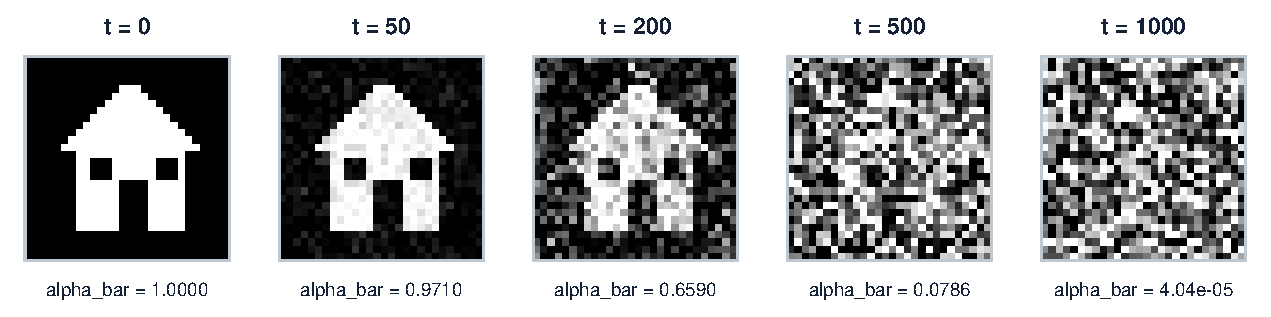
\includegraphics[width=\linewidth]{figures/noise_sequence.pdf}
\caption{Original forward-noising illustration at five timesteps.
The same trajectory is shown throughout. Values are clipped to $[-1,1]$
only for display; stored arrays and calculations remain unclipped.
The equation and schedule follow \cite{ho2020ddpm}.}\label{fig:noise}
\end{figure*}

\begin{table*}[t]
\centering\small
\caption{Coefficients computed by the supplied script. Signal and noise
columns refer to Eq.~\eqref{eq:closed}, not measured image quality.}
\label{tab:noise}
\begin{tabular}{@{}rrrrr@{}}
\toprule
$t$ & $\ab_t$ & Signal $\sqrt{\ab_t}$ & Noise SD $\sqrt{1-\ab_t}$ &
$\ab_t/(1-\ab_t)$\\
\midrule
0 & 1.000000 & 1.000000 & 0.000000 & $\infty$\\
50 & 0.971016 & 0.985401 & 0.170248 & 33.5015\\
200 & 0.659039 & 0.811812 & 0.583919 & 1.9329\\
500 & 0.078587 & 0.280334 & 0.959902 & 0.0853\\
1000 & 0.000040 & 0.006353 & 0.999980 & 0.000040\\
\bottomrule
\end{tabular}
\end{table*}
The last column is a schedule-based signal-to-noise coefficient ratio,
also a per-coordinate variance ratio for unit-variance data.
This illustrates corruption, not learned denoising or generation.

\section{LDM: Latent Space and Efficient Generation}\label{sec:ldm}
\subsection{Why move from pixels to a latent representation?}\label{sec:synthesis}
The diffusion framework supplies a way to generate images, but repeatedly processing a
high-resolution pixel grid is expensive. LDM separates learning a useful
image representation from learning its generative distribution
\cite[Secs.~3.1--3.2]{rombach2022ldm}. Its first stage compresses images;
its second stage applies diffusion to the resulting spatial tensors.
The central question is how much computation can be removed while
preserving information needed for convincing reconstruction.

A latent is a learned feature representation, not a smaller JPEG or a
text description. For RGB input $x_0\in\R^{H\times W\times3}$, let
$\tilde z\in\R^{h\times w\times c}$, where $h=H/f$, $w=W/f$,
$f\ge1$ is the spatial downsampling factor, and $c$ is the latent channel
count. For example, an LDM configuration with $f=4,c=3$ maps
$256\times256\times3$ to $64\times64\times3$
\cite[Table~8]{rombach2022ldm}. This reduces the number of spatial positions
by $16$, but the end-to-end runtime and memory depend on more than the
state shape.

\subsection{VAE encoder, decoder, and the compression trade-off}\label{sec:vae}
We emphasize LDM's KL-regularized, VAE-like autoencoder. Its encoder
predicts a distribution over representations of an input image
\cite{kingma2014vae,rombach2022ldm}:
\begin{align}
q_\phi(\tilde z\mid x_0)
 &=\Normal\!\left(\mu_\phi(x_0),\diag(\sigma_\phi^2(x_0))\right),\nonumber\\
\tilde z&=\mu_\phi(x_0)+\sigma_\phi(x_0)\odot\xi,\quad
\xi\sim\Normal(0,\Id),\nonumber\\
\hat x_0&=D_\psi(\tilde z).\label{eq:vae}
\end{align}
$\phi,\psi$ are encoder and decoder parameters. The encoder outputs
latent means $\mu_\phi$ and positive standard deviations $\sigma_\phi$;
$\diag$ forms a diagonal covariance and $\odot$ denotes elementwise
multiplication. The decoder $D_\psi$ reconstructs an image $\hat x_0$.
Reparameterization places randomness in $\xi$, enabling gradient-based
training. This posterior noise is different from the diffusion noise
added in the second stage.

The encoder must retain spatial and perceptual information; the decoder
must learn how to turn it back into image detail. Reconstruction quality
therefore limits what the complete generator can preserve. Excessive
compression may erase fine text, small objects, or textures that later
diffusion cannot faithfully restore.

Regularization makes the representation suitable for modeling, but the
first stage is not merely a textbook VAE with pixel reconstruction loss.
LDM uses perceptual and patch-adversarial reconstruction objectives with
a weak KL penalty \cite[Sec.~3.1]{rombach2022ldm}. Perceptual loss compares
visual features; adversarial training encourages locally realistic
texture. A textbook VAE objective is given in
Appendix~\ref{app:vaedetails} to distinguish these choices.
The original paper also studies VQ regularization, so LDM is broader than
this KL/VAE variant. Neither weak KL regularization nor successful
reconstruction makes clean encoded latents exactly standard normal.
The diffusion prior must still learn their distribution.

\subsection{Diffusion training and sampling in latent space}\label{sec:pipeline}
After the autoencoder is trained, its parameters are fixed while the
latent denoiser is trained. Let $z_0=a\tilde z$, with optional fixed scale
$a>0$ to match latent magnitudes to the noise schedule; $a=1$ means no
rescaling. Diffusion acts on $d_z=hwc$ latent coordinates:
\begin{align}
z_t&=\sqrt{\ab_t}\,z_0+\sqrt{1-\ab_t}\,\eps_z,\quad
\eps_z\sim\Normal(0,\Id_{d_z}),\label{eq:latentnoise}\\
L_{\rm LDM}&=\E_{x_0,y,t,\xi,\eps_z}
\left[\|\eps_z-\eps_\theta(z_t,t,\tau_\eta(y))\|_2^2\right].
\label{eq:ldmloss}
\end{align}
The condition $y$ may be a text prompt, encoded by $\tau_\eta$ with
parameters $\eta$. The time-conditioned denoiser, typically a U-Net,
returns a tensor of the same shape as $z_t$. The conditional objective
follows LDM \cite[Eq.~3]{rombach2022ldm}, here making stochastic encoding
explicit. Posterior-mean encoding omits $\xi$.

For generation, start with latent Gaussian noise and repeatedly apply a
compatible reverse sampler using the conditional predictor. Decode the
final latent once as $D_\psi(z_0/a)$, undoing the training scale.
Pure text-to-image generation needs no real input image or image encoder.
The encoder is needed to form training representations, whereas the
decoder converts a generated representation into pixels.
Figure~\ref{fig:ldm} makes these roles explicit.

\begin{figure*}[t]
\centering
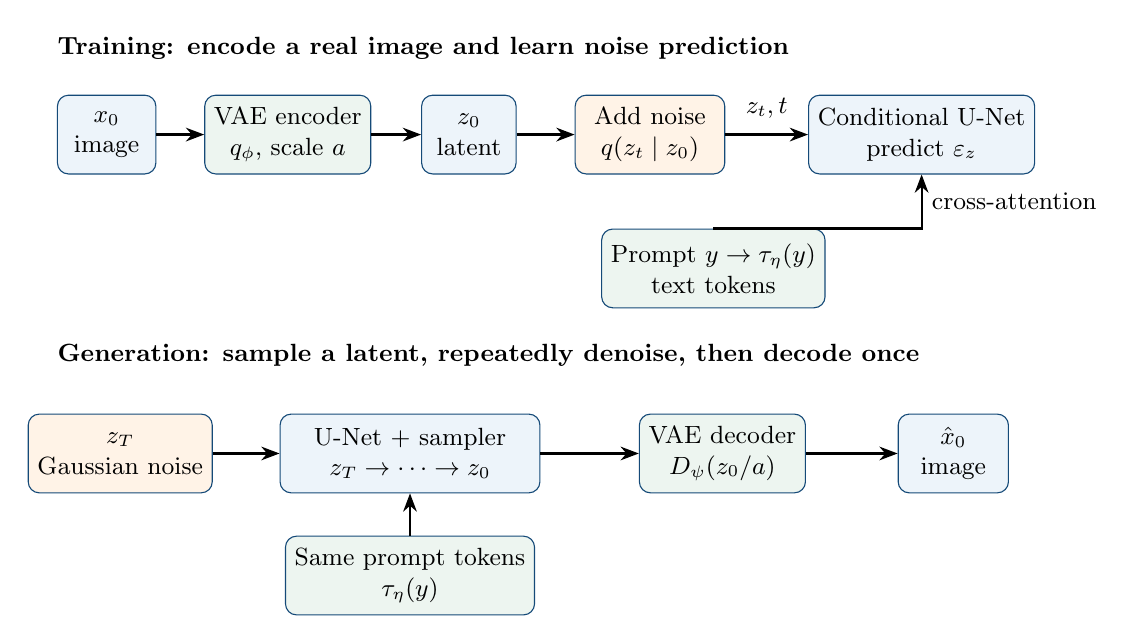
\begin{tikzpicture}[>=Stealth,x=1.15cm,
box/.style={draw=hcmusblue,rounded corners,fill=lightblue,
  align=center,font=\small,minimum height=1cm},
note/.style={font=\small,align=center}]
\node[note,anchor=west,font=\small\bfseries] at (0,3.8) {Training: encode a real image and learn noise prediction};
\node[box,minimum width=1.25cm] (x) at (.65,2.7) {$x_0$\\image};
\node[box,minimum width=1.9cm,fill=lightgreen] (e) at (2.65,2.7) {VAE encoder\\$q_\phi$, scale $a$};
\node[box,minimum width=1.2cm] (z) at (4.65,2.7) {$z_0$\\latent};
\node[box,minimum width=1.9cm,fill=lightorange] (q) at (6.65,2.7) {Add noise\\$q(z_t\mid z_0)$};
\node[box,minimum width=2.6cm] (u) at (9.65,2.7) {Conditional U-Net\\predict $\eps_z$};
\draw[->,thick] (x)--(e);
\draw[->,thick] (e)--(z);
\draw[->,thick] (z)--(q);
\draw[->,thick] (q)--node[midway,above=2pt,font=\small] {$z_t,t$}(u);
\node[box,fill=lightgreen,minimum width=2.6cm] (text) at (7.35,1) {Prompt $y\to\tau_\eta(y)$\\text tokens};
\draw[->,thick] (text.north) -| node[pos=.75,right,font=\small] {cross-attention}(u.south);
\node[note,anchor=west,font=\small\bfseries] at (0,-.1) {Generation: sample a latent, repeatedly denoise, then decode once};
\node[box,minimum width=1.5cm,fill=lightorange] (n) at (.8,-1.35) {$z_T$\\Gaussian noise};
\node[box,minimum width=3.3cm] (den) at (4,-1.35) {U-Net + sampler\\$z_T\to\cdots\to z_0$};
\node[box,minimum width=2cm,fill=lightgreen] (dec) at (7.45,-1.35) {VAE decoder\\$D_\psi(z_0/a)$};
\node[box,minimum width=1.4cm] (out) at (10,-1.35) {$\hat x_0$\\image};
\draw[->,thick] (n)--(den);
\draw[->,thick] (den)--(dec);
\draw[->,thick] (dec)--(out);
\node[box,fill=lightgreen,minimum width=2.6cm] (gentext) at (4,-2.9) {Same prompt tokens\\$\tau_\eta(y)$};
\draw[->,thick] (gentext.north)--(den.south);
\end{tikzpicture}
\caption{Original latent diffusion pipeline, based on
\cite[Fig.~3 and Sec.~3]{rombach2022ldm}. The VAE is learned first and
frozen for diffusion training; its decoder runs after the denoising loop.
Pure text-to-image generation does not require a real input image or the
image encoder.}\label{fig:ldm}
\end{figure*}

\subsection{Conditioning and the complete pipeline}\label{sec:attention}\label{sec:cfg}
LDM uses cross-attention to make denoising depend on a condition such as
text \cite[Sec.~3.3]{rombach2022ldm}. Spatial image features supply
queries; prompt-token embeddings supply keys and values. Learned
attention weights retrieve text information useful for the current
features. Thus a prompt changes the denoising predictions throughout
the sampling loop; it is not pasted onto the decoded image.
The matrix formulation and an optional toy calculation are confined to
Appendix~\ref{app:attention}.

Classifier-free guidance can strengthen conditional influence by using
$\eps_u+s(\eps_c-\eps_u)$, where $\eps_u,\eps_c$ are unconditional and
conditional predictions and $s\ge0$ is the guidance scale
\cite{ho2022cfg}. Here $s=1$ is ordinary conditional sampling.
Stronger guidance can trade diversity for conditional fidelity; it does
not guarantee correct counting, spatial relations, or attribute binding.
Standard CFG uses two denoiser evaluations per step. Details are in
Appendix~\ref{app:cfg}.

The two papers therefore address complementary questions: DDPM learns
how iterative denoising can generate an image distribution; LDM learns
a representation in which that iteration is less expensive. Compression
reduces repeated spatial work. Faster samplers such as DDIM instead
reduce the number of evaluations \cite{song2021ddim}; the two ideas can
be combined without treating them as the same speedup.

\section{Results and Discussion}\label{sec:results}

\subsection{Experimental setup and sampling speed}\label{sec:tradeoffs}
We ran pretrained diffusion checkpoints in Google Colab on an NVIDIA
Tesla T4. The LSUN Churches run compares two unconditional generators at
$256\times256$: Google DDPM in pixel space and CompVis LDM-KL-8 in latent
space. Both used DDIM with 50 updates, $\eta=0$, float32, batch size one,
and seeds 2026--2029. After one warm-up per model, we measured elapsed
time from sampling the initial noise to producing an RGB tensor,
synchronizing the GPU before recording the time. The timing includes the
LDM decoder and excludes checkpoint loading and PNG export.

\begin{table}[t]
\centering\small
\caption{Our LSUN Churches comparison. Latency is the median of four
images. Memory is peak CUDA tensor allocation reported by PyTorch.}
\label{tab:comparison}
\begin{tabularx}{\columnwidth}{@{}Ycc@{}}
\toprule
Criterion & Pixel DDPM & LDM-KL-8\\
\midrule
Denoising state & $256\times256\times3$ & $32\times32\times4$\\
Latency (s/image) & 6.10 & 2.44\\
Peak allocation (GiB) & 0.75 & 1.68\\
\bottomrule
\end{tabularx}
\end{table}

The latent pipeline achieved a $2.50\times$ speedup in median sampling
time and used more peak tensor memory (Table~\ref{tab:comparison}).
A smaller denoising state reduces the spatial grid processed at each
update, while model weights, intermediate activations, and the decoder
also contribute to memory. The checkpoints and software implementations
differ, so the measurements compare these two pipelines under the
recorded settings.

\subsection{ImageNet samples and denoising trajectories}
\label{sec:imagenet-results}
A separate run compared OpenAI's class-conditional ADM in pixel space
with CompVis \texttt{cin256-v2}, a VQ-regularized LDM with a
$64\times64\times3$ latent. Each model generated one $256\times256$
image per class using seed 2026 and 50 deterministic DDIM updates
($\eta=0$). Both used the same class IDs. LDM additionally used
classifier-free guidance with scale $3.0$. Figure~\ref{fig:imagenet-grid}
shows all ten final images.

\begin{figure*}[t]
\centering
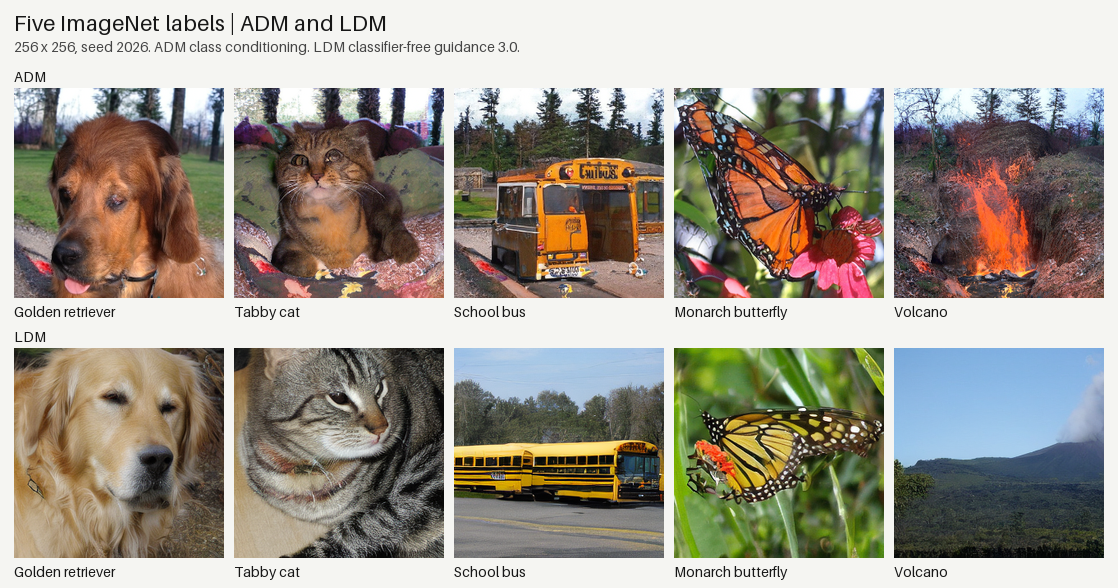
\includegraphics[width=0.94\textwidth]{figures/colab/imagenet_comparison.png}
\caption{Our ImageNet samples for five shared class labels. The top row
uses pixel-space ADM and the bottom row uses latent diffusion.}
\label{fig:imagenet-grid}
\end{figure*}

\begin{figure*}[t]
\centering
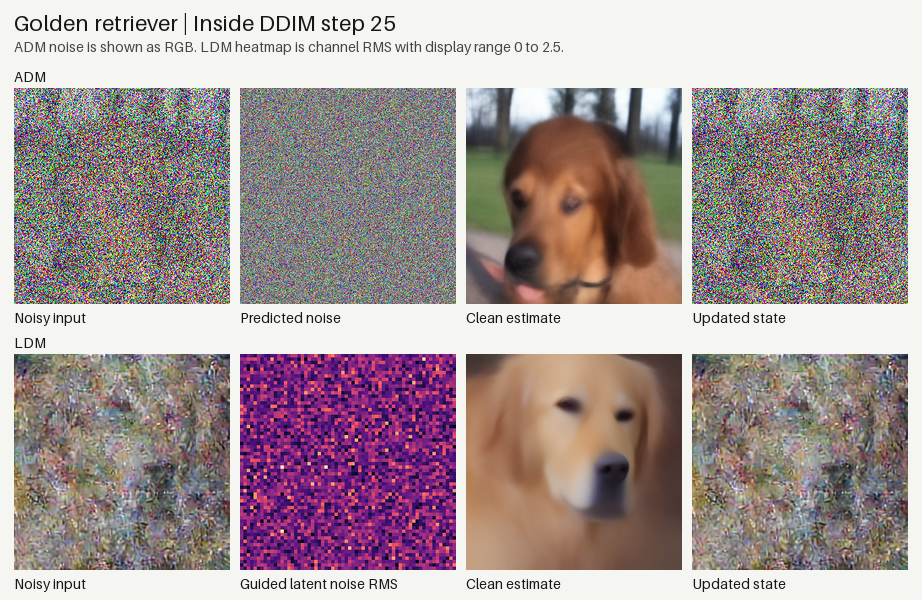
\includegraphics[width=0.88\textwidth]{figures/colab/retriever_step25.png}
\caption{Inside DDIM update 25 for the golden retriever. Read each row
from the noisy input through the predicted noise and clean estimate to
the updated state. ADM noise is displayed in RGB. The LDM heatmap
shows the root mean square of the guided noise across latent channels.
The other LDM panels show decoded states.}
\label{fig:imagenet-step}
\end{figure*}

Reverse sampling starts from a Gaussian draw. At each update the
denoiser predicts noise, the sampler estimates the clean state, and
that estimate helps compute the next state. At update 25, the clean
estimates already show the retriever's head and muzzle, while the
updated states still carry visible noise (Figure~\ref{fig:imagenet-step}).
In a separate forward pass, we start from each model's final state
and add Gaussian noise using its schedule. The retriever's features
gradually disappear. Appendix~\ref{app:colab-traces} shows both
directions for all five labels.

We assess these samples visually by looking for class features and
coherent shapes. Both bus samples show yellow bodies and rows of
windows. The volcano appears as a lava scene in ADM and as a slope
with a plume in LDM. The different outputs illustrate variation
under the same label. One sample per class and different guidance
settings limit the comparison to the examples shown.

\subsection{Published evidence on quality and speed}\label{sec:benchmark}
For a quantitative comparison within one task, Rombach
et al.~\cite[Table~6]{rombach2022ldm} report $0.26$ versus $0.97$
samples/s at $256^2$ and FID@2k $24.74$ versus $15.21$ after six epochs
for pixel LDM-1 and latent LDM-4 (KL with attention), respectively,
in Places inpainting. FID compares generated and reference feature
distributions \cite{heusel2017fid}. These figures describe the paper's
inpainting setup.

\paragraph{DDPM objective ablation.}
On unconditional CIFAR-10, Ho et al.~\cite[Tables~1--2]{ho2020ddpm}
report training-reference FID of $13.51$ for the variational objective
and $3.17$ for the simplified objective with epsilon prediction and
fixed isotropic variance. The reported NLL upper bound changes from
$3.70$ to $3.75$ bits per dimension.

\FloatBarrier
\subsection{Prompt control, training data, copyright, and bias}
\label{sec:ethics}
\textbf{Prompt-based control.} A text prompt can specify a subject,
attributes, or spatial relations. In a text-conditioned diffusion model,
cross-attention lets image features use information from the prompt.
Classifier-free guidance can strengthen conditioning at the cost of
diversity \cite{rombach2022ldm,ho2022cfg}. Our ImageNet run tests generation
from class labels. Free-form attributes and relations require a separate
prompt-adherence evaluation.

\textbf{Training data and bias.} Dataset coverage and, for text-to-image
models, caption quality affect which subjects and relations a model
learns. Our checkpoints cover church imagery or the ImageNet label
vocabulary. Bianchi et al.~\cite{bianchi2023bias} found demographic stereotypes
in outputs for ordinary prompts. Our five classes and four church seeds
provide too little coverage for a bias audit.

\textbf{Copyright and memorization.} Carlini et al.~\cite{carlini2023extract}
extracted memorized training images from diffusion models. This motivates
documenting data provenance and checking for close matches to training
images. Permissions for training materials and rights in generated outputs
are separate questions. The U.S. Copyright Office report discusses
training under U.S. copyright law \cite{usco2025training}.

\section{Conclusion}\label{sec:conclusion}
Learning to remove noise enables generation by fitting a sequence of
reverse conditional distributions. The 2015 diffusion framework supplies
forward Gaussian corruption, learned reverse mean/covariance functions,
and variational training against tractable posterior targets. Starting
from a new Gaussian draw and composing the reverse transitions then
produces an image sample. DDPM retains this construction while fixing
variance choices, parameterizing the reverse mean through predicted
noise, and simplifying the training objective. Its published ablation
supports a sample-quality benefit from that objective choice, distinct
from likelihood optimization or fewer sampling steps. The score
connection explains the parameterization without adding a separate
computational stage.


LDM preserves this denoising principle in a learned representation.
The ImageNet traces show recognizable structure emerging in both spaces.
In our LSUN Churches run, the latent pipeline had lower sampling latency
and higher peak tensor allocation. These measurements apply to the tested
checkpoints. Text control and the effects of training data require
evaluation beyond class-conditioned image examples.

\FloatBarrier
\label{LastBodyPage}
\clearpage
{\small
\balance
\bibliographystyle{ieeenat_fullname}
\bibliography{references}
}
\clearpage
\nobalance
\appendix
\twocolumn[{
\section{Requirement-to-Evidence Map}\label{app:map}
This map concerns the written report. The assignment's separate slide,
oral-presentation, balanced-participation, and Q\&A requirements require
presentation deliverables and cannot be fulfilled by a report alone.
The main text occupies pages 1--\pageref{LastBodyPage};
references and appendices are separate.

\begin{center}
\begin{minipage}{\textwidth}
\centering\small
\captionsetup{hypcap=false}
\captionof{table}{Coverage of the supplied CS420 S06 seminar brief.}
\begin{tabularx}{\linewidth}{@{}p{1.1cm}YY@{}}
\toprule
Task & Required content & Location / evidence\\
\midrule
1 & Generative versus discriminative; GAN, autoregressive, diffusion &
Sections~\ref{sec:families}, \ref{sec:generator-comparison};
Table~\ref{tab:families}\\
2 & Forward process, beta schedule, Gaussian noise, noise predictor,
reverse sampling; both-direction diagram &
Section~\ref{sec:ddpm}; Eqs.~\eqref{eq:forward}--\eqref{eq:reverse};
Figure~\ref{fig:ddpm}\\
3 & Manual 1D forward step, symbols, stochastic expectation &
Section~\ref{sec:scalar}; $x_1=0.600833$; conditional mean and variance\\
4 & Small image at five noise levels; optional pretrained demonstration &
Section~\ref{sec:noise}; Figure~\ref{fig:noise}; Table~\ref{tab:noise};
executable code and arrays. Pretrained generation was not performed\\
5 & VAE encoder/decoder, latent operations, cross-attention, pipeline &
Sections~\ref{sec:vae}--\ref{sec:attention};
Eqs.~\eqref{eq:vae}--\eqref{eq:attention};
Figures~\ref{fig:ldm}--\ref{fig:attention}\\
6 & Speed, quality, prompt control, data, copyright, bias;
explicit pixel/latent comparison &
Sections~\ref{sec:cfg}, \ref{sec:benchmark}--\ref{sec:ethics};
Tables~\ref{tab:benchmark}--\ref{tab:comparison}\\
\bottomrule
\end{tabularx}
\end{minipage}
\end{center}
\vspace{8pt}
}]


\textbf{Required representations.}
Equation~\eqref{eq:forward} is the Gaussian forward transition;
Eq.~\eqref{eq:loss} is the simplified noise-prediction objective.
The worked example gives a complete substitution, result, and interpretation.
Appendix~\ref{app:notation} records ranges, units, and modeling assumptions.

\textbf{Paper reading and synthesis.}
DDPM's forward/reverse method and contribution are reviewed in
Section~\ref{sec:ddpm}. LDM's representation, method, conditioning,
contributions, and differences are developed in
Sections~\ref{sec:ldm}--\ref{sec:synthesis}.
Section~\ref{sec:benchmark} identifies the exact source table for performance
claims. The report includes Abstract, Introduction, Background/Paper Review,
Method/Worked Example, Results and Discussion, Conclusion, and References.
English is used according to the commissioning instruction, which overrides
the brief's Vietnamese-language request.

\pagecut
\section{Reproducibility, Evaluation Protocol, and Attribution}\label{app:repro}
\subsection{Reproduce the original illustration}
The Overleaf project already contains the generated figure; Python is not
needed to compile the report. To regenerate it locally:
\begin{lstlisting}[language=bash]
python -m pip install -r code/requirements.txt
python code/make_figures.py
latexmk -pdf -interaction=nonstopmode -halt-on-error main.tex
\end{lstlisting}
The figure uses a synthetic geometric image, not MNIST or another dataset.
The script records the seed, schedule coefficients, library versions,
scalar example, and benchmark-ratio arithmetic in
\texttt{figures/analysis.json}. It saves unclipped frames, timesteps, the
schedule, and cumulative coefficients in \texttt{noise\_arrays.npz},
and summary coefficients in \texttt{noise\_levels.csv}.
The delivered run used NumPy 2.3.5 and ReportLab 4.4.9.
The sequence is one sampled Markov path; identical seeds and library
versions reproduce it. No image-generation checkpoint is involved.

\subsection{A future prompt and runtime study (not executed)}
Select and record exact checkpoint identifiers, revisions, dataset licenses,
hardware, software versions, numerical precision, resolution, and batch
size. Keep each fixed within a comparison and record warm-up policy.
For latent models, measure text encoding, denoising, decoding, and
end-to-end latency separately, and record peak allocated memory over the
entire pipeline.

Use paired prompts such as \emph{a red cube to the left of a blue sphere}
and \emph{a green cube to the left of a blue sphere}; separately swap the
spatial relation. Predefine at least 20 seeds per condition and inspect
all samples. Vary sampling steps and guidance in separate sweeps.
Report object presence, color binding, relation correctness, and diversity;
do not select only attractive examples. This is a proposed evaluation
design, not empirical evidence of a model's prompt capability.

\subsection{Provenance and AI assistance}
Figures~\ref{fig:ddpm}, \ref{fig:ldm}, and \ref{fig:attention} are original
TikZ schematics explaining cited methods; no paper figure is reproduced.
Figure~\ref{fig:noise} and Table~\ref{tab:noise} are generated by the supplied
code. Table~\ref{tab:benchmark} is transcribed from LDM Table~6; ratios are
our arithmetic. The two qualitative comparison tables are analytical
syntheses with sources in their captions.

The document uses the requested ICCV 2025 author kit
\cite{template}, with its official style and bibliography files.
It uses 10-point type, two columns, and US Letter paper, following the
new template request. The author block retains HCMUS and CS420 information
and three name/ID placeholders. Template provenance is included in the project.

OpenAI Codex \cite{codex} assisted with drafting, equations, code,
diagram construction, source checking, and LaTeX preparation.
Preparation checks included consulting the original DDPM/LDM equations and
LDM Table~6, recalculating the numerical examples and ratios, and compiling
and visually reviewing the PDF. The named student authors should review
and accept the final manuscript and replace the author placeholders before
submission. No human study, new trained model, or pretrained generation
benchmark is claimed.

\pagecut
\twocolumn[{
\section{Notation, Assumptions, and Additional Derivation}\label{app:notation}
\subsection{Ranges and units}
Images are normalized and dimensionless. Clean pixels in the illustration
lie in $[-1,1]$; noisy states, latent values, and predicted noise are
real-valued and need not stay within that interval.
There is no physical time unit in the diffusion index.

\begin{center}
\begin{minipage}{\textwidth}
\centering\small
\captionsetup{hypcap=false}
\captionof{table}{Notation used in the equations; meanings are also introduced
beside the corresponding equations in the main text.}
\begin{tabularx}{\linewidth}{@{}p{3.3cm}Y@{}}
\toprule
Symbols & Meaning, range, and units\\
\midrule
$x_0,x_t,\hat x_0$ & Clean/noisy/reconstructed image; vector in $\R^D$ or
an equivalent image tensor; normalized intensity units\\
$D,H,W,h,w,c,d_z$ & Positive integer dimensions. $D=3HW$ for RGB,
$d_z=hwc$; $H,W$ count pixels, $h,w$ count latent positions\\
$t,T,j$ & Integer timestep, terminal step, and product index;
$1\le t\le T$, $1\le j\le t$\\
$\beta_t,\alpha_t,\ab_t$ & Dimensionless schedule coefficients;
$0<\beta_t<1$, $\alpha_t=1-\beta_t$, $0<\ab_t\le1$\\
$q,p_\theta,p_{\rm data}$ & Fixed forward transition, learned reverse/generative
distribution, and data distribution, respectively\\
$\Normal(\mu,\Sigma),\Id$ & Gaussian with mean $\mu$ and covariance $\Sigma$;
identity covariance of the relevant dimension\\
$\eps,\eps_z,u,\xi$ & Independent standard-normal draws in their respective
sampling operations; each coordinate has mean $0$ and variance $1$\\
$\sigma_t,\mu_\phi,\sigma_\phi$ & Reverse noise standard deviation
$\sigma_t\ge0$; VAE posterior mean and positive standard deviations\\
$\theta,\phi,\psi,\eta,\omega$ & Trainable parameter arrays of denoiser,
VAE encoder, decoder, condition encoder, and illustrative classifier\\
$\tilde z,z_0,z_t,f,a$ & Raw/clean-scaled/noisy latent;
spatial factor $f\ge1$, with $H,W$ divisible by $f$;
fixed dimensionless scale $a>0$\\
$y,\tau_\eta(y),F,C$ & Condition, encoded condition, U-Net features, and token
embedding matrix. Continuous embeddings are real-valued\\
$n,m,d_u,d_y,d_a,d_v$ & Positive integer counts and widths for cross-attention;
see Section~\ref{sec:attention} for all matrix shapes\\
$Q,K,V,A,O$ & Query, key, value, attention-weight, and output matrices;
$A_{ij}\in[0,1]$ and $\sum_j A_{ij}=1$\\
$s,w,p_{\rm drop},\varnothing$ & CFG scale $s\ge0$, alternative scale $w=s-1$,
dropout probability in $(0,1)$, and null condition\\
$K,r,\mathcal T$ & In the cost model only, $K$ counts updates (not attention
keys), $r$ counts evaluations/update, and $\mathcal T$ is seconds\\
$L_{\rm simple},L_{\rm LDM}$ & Expected summed squared noise-prediction
errors; dimensionless squared normalized-coordinate units\\
$\E,\|\cdot\|_2,\KL$ & Expectation, Euclidean norm, and KL divergence;
natural logarithms make KL and negative log likelihood use nats\\
\bottomrule
\end{tabularx}
\end{minipage}
\end{center}
\vspace{8pt}
}]


\pagecut
\subsection{Why the forward marginal is available in closed form}
Assume independent standard-normal innovations
$\eps^{(1)},\eps^{(2)}$ and let $x_0$ be fixed. Applying
Eq.~\eqref{eq:forward} twice gives
\begin{align*}
x_1&=\sqrt{\alpha_1}x_0+\sqrt{\beta_1}\eps^{(1)},\\
x_2&=\sqrt{\alpha_2\alpha_1}x_0
+\sqrt{\alpha_2\beta_1}\eps^{(1)}
+\sqrt{\beta_2}\eps^{(2)}.
\end{align*}
The two independent noise terms have total variance
$\alpha_2\beta_1+\beta_2
=\alpha_2(1-\alpha_1)+(1-\alpha_2)=1-\alpha_2\alpha_1$.
A sum of independent Gaussians is Gaussian. Repeating this argument yields
Eq.~\eqref{eq:closed}, with mean $\sqrt{\ab_t}x_0$ and covariance
$(1-\ab_t)\Id$ \cite{ho2020ddpm}.

Gaussian innovations are independent across coordinates and steps, but
the noisy images themselves have correlations inherited from $x_0$.
When $\ab_T$ is close to zero, dependence on the starting image is weak
and a standard-normal starting prior is a useful approximation.
A finite schedule need not make it exactly equal to that prior.
The learned Gaussian reverse transition is a modeling approximation
motivated by small forward steps; no finite network is assumed to know
the exact reverse conditional.

\subsection{Why noise prediction is useful without knowing the true noise}
For a fixed $x_t$ and $t$, the vector minimizing expected squared prediction
error is $\E[\eps\mid x_t,t]$ (and, in a conditional model,
$\E[\eps\mid x_t,t,y]$). Thus a trained predictor estimates a statistical
direction shared by plausible clean examples, not an oracle that recovers
every random draw. Its corresponding clean-state estimate is
\begin{equation}
\hat x_0(x_t,t)=
\frac{x_t-\sqrt{1-\ab_t}\eps_\theta(x_t,t)}{\sqrt{\ab_t}}.
\end{equation}
This follows by rearranging Eq.~\eqref{eq:closed}; prediction errors remain
and can be magnified at small $\ab_t$. The reverse sampler uses predictions
over many levels rather than treating one estimate as guaranteed recovery.
The same argument applies in latent space, followed by the learned decoder.

\subsection{Two training stages and their different roles}
Stage one updates encoder $\phi$ and decoder $\psi$ to preserve useful
image information in a regularized representation. Stage two fixes them
and trains denoiser $\theta$ with Eq.~\eqref{eq:ldmloss}. The original LDM
conditional formulation jointly optimizes the condition encoder and
denoiser \cite[Sec.~3.3]{rombach2022ldm}; particular later implementations
may instead keep the text encoder fixed.

The distinction matters: improving the denoiser cannot guarantee exact
recovery of details that the first stage systematically discards.
Conversely, a high-quality autoencoder does not itself provide the
conditional latent distribution needed for generation. The VAE prior
regularizer and the learned diffusion prior play different roles.

\end{document}
